\section{D-Optimal Designs Without Model Error}\label{section:vanishing}
Our goal in this section is to prove Theorem \ref{thm:char} which
characterizes D-optimal designs when $\modcov = 0$. The necessary
first-order condition for D-optimality of Theorem
\ref{thm:constrained} for $\modcov = 0$ become:

\begin{equation}\label{eq:eigenproblem}
  \sigma^{-2}\fwd \postcov \fwd^* \obs^* = \obs^* \Xi,
\end{equation}
with $\Xi$ diagonal. Equation \eqref{eq:eigenproblem} looks like an
eigenvalue problem for the self-adjoint operator $\sigma^{-2}\fwd
\postcov \fwd^*$, where rows of $\obs$, namely $\meas_j,j=1,\dots, m$,
are eigenvectors. However, $\postcov$ depends on $\obs$, so we refer
to \eqref{eq:eigenproblem} as a \emph{nonlinear} eigenvalue problem.
%% Proposition \ref{prop:twice_woodbury} and Lemma \ref{lemma:sim
%%_diag} required

\begin{proposition}\label{prop:twice_woodbury}
  Assume $\fwd \prcov \fwd^*$ is invertible. Then
  \begin{align*}
    \begin{split}
      \fwd( \prcov^{-1} + \sigma^{-2}  \fwd^* \obs^* \obs \fwd )^{-1} \fwd^* 
      %
      %
      = \left ( (\fwd\prcov\fwd^*)^{-1} + \sigma^{-2}  \obs^* \obs \right )^{-1},
    \end{split}
  \end{align*}  
\end{proposition}

As we mentioned in Section \ref{subsec:bayesian_inverse_problems},
$\fwd \prcov \fwd^*$ is the prior covariance in $\hilo$ and could be
safely assumed invertible. The proof of Proposition
\ref{prop:twice_woodbury} is delegated to the Supplementary. It
amounts to using Woodbury's matrix identity twice. The standard proof
for Woodbury's matrix identity works for separable Hilbert spaces, as
long as all terms are well defined. Unfortunately, $\obs^*\obs$ is not
invertible, so we utilize a regularization trick to force it to be.

\begin{lemma}[Simultaneous diagonalizability]\label{lemma:sim_diag}
  Let $\hil$ separable Hilbert space, $C:\hil \to \hil$ self-adjoint
  and $\func_1,\dots,\func_m \in \hil$. Denote $\func^*$ the element
  $\func$ acting as a linear functional. If
  \begin{equation*}
   (C + \sum_{j=1}^m \func_j\func_j^*) \func_l = \xi_l \func_l,\ l = 1,\dots,m
  \end{equation*}
  then $C$ and $\sum_{j=1}^m \func_j \func_j^*$ are simultaneously
  diagonalizable.
\end{lemma}
The proof of Lemma \ref{lemma:sim_diag} is delegated to the
Supplementary.

\begin{proposition}\label{prop:same_ev}
  Let $\obs$ satisfy the nonlinear eigenvalue problem
  \eqref{eq:eigenproblem}. Then $\obs^*\obs$ and $\fwd \prcov \fwd^*$
  are simultaneously diagonalizable.
\end{proposition}
\begin{proof}
  \begin{align}\label{eq:mod_conditions}
    \begin{split}
      \obs^* \Xi &= \sigma^{-2}\fwd \postcov \fwd^* \obs^*  \text{ (by \eqref{eq:eigenproblem})}\\
      %
      %
      %
      &= \sigma^{-2} \fwd( \prcov^{-1} + \sigma^{-2}  \fwd^* \obs^* \obs \fwd )^{-1} \fwd^* \obs^*  \text{ (by \eqref{eq:postcov})} \\
      %
      %
      %
      &= \sigma^{-2} \left ( (\fwd\prcov\fwd^*)^{-1} + \sigma^{-2}  \obs^* \obs \right )^{-1} \obs^* \text{ (by Proposition \ref{prop:twice_woodbury})}.
    \end{split}
  \end{align}

  Now take $\func_j^{*} = \meas_j$ and $C := (\fwd \prcov
  \fwd^*)^{-1}$ and use Lemma \ref{lemma:sim_diag}.
\end{proof}

Since we made no assumption regarding the ordering of $\{\lambda_i\}$,
we can denote the corresponding non-zero eigenvalues of $\obs^*\obs$
by $\{\eta_i\}_{i=1}^{k}$ and let $\eta_i = 0$ for $i \geq k+1$.

\begin{proposition}\label{prop:true_target}
  Let $\obs$ with $m$ measurements satisfy the nonlinear eigenvalue
  problem \eqref{eq:eigenproblem}. Let $\{\eta_i\}_{i=1}^{\infty}$
  eigenvalues of $\obs^*\obs$ and $\{\lambda_i\}_{i=1}^{\infty}$ the
  corresponding eigenvalues of $\fwd \prcov \fwd^*$. Let $k:=\rank
  \obs^*\obs$. Without loss of generality, let $\eta_i > 0$ for $i\leq
  k$ and $\eta_i = 0$ for $i > k$. Then:
  \begin{enumerate}
    \item $k \leq m$ and $\obs^*\obs$ has exactly $k$ positive
      eigenvalues.
    \item
      \begin{equation*}
        \tar(\obs) = \frac12 \sum_{i=1}^{k} \log (1 + \sigma^{-2}\lambda_i\eta_i) = \frac12 \sum_{i=1}^{m} \log (1 + \sigma^{-2}\lambda_i\eta_i).
      \end{equation*}
    \item Furthermore, if $\obs$ is D-optimal, $\eta_i > 0$ for
      eigenvectors corresponding to the $k$ largest $\lambda_i$.
  \end{enumerate}
\end{proposition}
\begin{proof}
  Part (1) is trivial. To see part (2) holds: 
  \begin{align}
    \begin{split}
      \tar(\obs) &= \frac12\log \det \left (I + \sigma^{-2} \prcov^{1/2} \fwd ^* \obs^*
      \obs \fwd \prcov^{1/2}\right )\\% \text{ (by definition)}\\
      %
      &= \frac12 \log \det \left (I + \sigma^{-2} \obs^* \obs \fwd
      \prcov\fwd^* \right ) \text{ (Sylvester's Determinant
      Theorem)}\\
      %
      %
      %
      &=\frac12 \log \prod_{i=1}^{\infty} ( 1 + \sigma^{-2} \lambda_i\eta_i ) \text{ (Proposition \ref{prop:same_ev})} \\
      %
      %
      %
      %&=\frac12 \log \left ( \prod_{i=1}^{k} ( \lambda_i^{-1} + \sigma^{-2} \eta_i )\prod_{i=1}^{k} \lambda_i \right )
      %
      %
      %
      &=\frac12 \sum_{i=1}^{k} \log (1 + \sigma^{-2}\lambda_i\eta_i). 
      %
      %
      %% &=\frac12 \sum_{i=1}^{k} \log(\sigma^2\lambda_i^{-1} + \eta_i) - k\log \sigma + \frac12\sum_{i=1}^k \log \lambda_i.
    \end{split}
  \end{align}
  Part (3) holds since $\log$ is increasing and $\eta_i \geq 0$.
\end{proof}


\begin{proposition}\label{prop:kkt}
  Let $\tar: \mathbb{R}^m \to \mathbb{R}$, $\tar(\eta) =
  \frac{1}{2}\sum_{i=1}^m \log (1+\sigma^{-2}\lambda_i \eta_i)$, with
  $\lambda_i > 0$ and $\sigma^{2} > 0$. Then the maximum of $\tar$
  subject to $\eta_i \geq 0$ and $\sum\eta_i = m$ is obtained at
  \begin{equation}
  \eta_i = \begin{cases}
    \frac{m}{k} - \sigma^2 \lambda_i^{-1} + \sigma^2 \frac{1}{k} \sum_{j\in A} \lambda_j^{-1} & i \in A \\
    0 & i \in A^c
  \end{cases}
  \end{equation}
  where $A:= \{1\leq i \leq m: \eta_i > 0\}$ and $A^c = \{1,\dots, m\}
  \backslash A$, and $k = |A|$, the cardinality of $A$.
\end{proposition}

The proof of Proposition \ref{prop:kkt} amounts to utilizing the
Karush-Kuhn-Tucker conditions and is delegated to the
Supplementary. The final ingredient we require for the proof of
Theorem \ref{thm:char} characterizing D-optimal designs is:


\begin{lemma}[Unit norm decomposition]\label{lemma:free}
  Let $M \in \R^{k \times k}$ symmetric positive definite with $\ttr M
  = m$, $m \geq k$. We can find $\func_j \in \R^k,j=1,\dots,m$
  with $\|\func_j\|=1$ and $A = (\func_1,\dots,\func_m)$ such that
  $AA^t = M$.
\end{lemma}

The proof of Lemma \ref{lemma:free} is also delegated to the
Supplementary. It is however important to note that this proof is
constructive; it will allow us to construct D-optimal designs, once we
fully characterize them in Theorem \ref{thm:char} below.


\begin{theorem}\label{thm:char}
  Let:
  \begin{itemize}
    \item The D-optimality design criterion
    \cite{AlexanderianGloorGhattas14}:
    \begin{align*}
      \begin{split}
        \tar(\obs) %:&= \mathbb{E}_{\data}\left [ D_{\text{KL}} (\post || \pr ) \right ] \\
        % 
        % 
        % 
        &= \frac12 \log \det ( I + \sigma^{-2} \prcov^{1/2} \fwd ^*
        \obs^* \obs \fwd \prcov^{1/2}), 
      \end{split}
    \end{align*}
  \item \(\opt\) a D-optimal design operator
    \begin{equation*}
      \opt = \argmax_{\|\meas_j\| = 1, j=1,\dots,m}\tar(\obs),
    \end{equation*}
  \item \(\{\lambda_i\}_{i=1}^\infty\) eigenvalues of
    \(\fwd\prcov\fwd^*\) in decreasing order of magnitude.
    %% \item \(\{\ev_i\}_{i=1}^\infty\) their corresponding eigenvectors.
  \item \(\{\eta_i\}_{i=1}^\infty\) eigenvalues of \(\opt^*\opt\).
 
  \end{itemize}

  Then:
  \begin{enumerate}
  \item  \(\tr{\opt^*\opt} = m\).
  \item \(\opt^*\opt\) and \(\fwd\prcov\fwd^*\) are simultaneously
    diagonalizable.
  \item \(k := \rank \opt^*\opt \leq m\) and
    \begin{equation*}
      \tar(\opt) = \frac12 \sum_{i=1}^{k} \log (1 + \sigma^{-2}\lambda_i\eta_i). %= \frac12 \sum_{i=1}^{m} \log (1 + \sigma^{-2}\lambda_i\eta_i).
    \end{equation*}
  %% \item 
  %%   \begin{equation*}
  %%     k = \argmax \left \{ k:\lambda_k^{-1} < \sigma^{-2}\frac{m}{k} + \frac{1}{k} \sum_{j=1}^{k}
  %%     \lambda_j^{-1} \right \}.
  %%   \end{equation*}
  \item
    \begin{equation*}
        \eta_i = \begin{cases}
          \frac{m}{k} - \sigma^2 \lambda_i^{-1} + \sigma^2 \frac{1}{k} \sum_{j=1}^k \lambda_j^{-1} & 1 \leq i \leq k \\
          0 & i > k 
        \end{cases}.
    \end{equation*}
  \item The covariance of the pushforward \(\fwd_{*} \postopt\) is \(\left
    ( (\fwd \prcov \fwd^*)^{-1} + \sigma^{-2} \opt^*\opt \right
    )^{-1}\) and its eigenvalues are
    \begin{equation}\label{eq:cylinders}
      \theta_i =
      \begin{cases}
        \left(\frac{\sum_{j=1}^k \lambda_j^{-1} + \sigma^{-2}m}{k} \right )^{-1} & i \leq k \\
        \lambda_i &  i > k 
      \end{cases}.
    \end{equation}
  \end{enumerate}
\end{theorem}

\begin{proof}
  Part (1) is immediate for any measurement operator $\obs$ that
  satisfies the unit norm constraint on measurements. Part (2)
  was proved in Proposition \ref{prop:same_ev}. Part (3) was proved in
  Proposition \ref{prop:true_target}.
  
  Part (4) is a consequence of Propositions \ref{prop:true_target} and
  \ref{prop:kkt}, with the caveat that we did not show that finding
  $\opt$ so that $\opt^*\opt$ has the desired eigenvalues is
  feasible. To this end, we utilize Lemma \ref{lemma:free}: let $M =
  \diag(\eta_1, \dots, \eta_k)$, diagonal with respect to the first
  $k$ eigenvectors of $\fwd \prcov \fwd^*$. We take $\opt := A$ from
  Lemma \ref{lemma:free}.
  
  Recall from \eqref{eq:postcov}, that the posterior precision is
  $\postcov^{-1} = \prcov^{-1} + \sigma^{-2}\fwd^*\opt^*\opt\fwd$. The
  first statement in part (5) now follows from Proposition
  \ref{prop:twice_woodbury}, while the second statement follows from
  parts (1) and (4).
\end{proof}


\pgfplotstableread{
  Label     prior  optimal  sub-optimal 
  1         0.2    1.8           1.7
  2         0.8    1.2           0.8
  3         2.2    0             0.5
  4         3.5    0             0.0
}\optimalvsnot

\begin{figure}\label{fig:tikz_clusterization}
  \centering
  \begin{tikzpicture}[scale=0.75]
    \begin{axis}[
        ybar stacked,
        ymin=0,
        ymax=4,
        xtick=data,
        legend style={cells={anchor=east}, legend pos=north west, legend columns=-1},
        reverse legend=false, % set to false to get correct display, but I'd like to have this true
        xticklabels from table={\optimalvsnot}{Label},
        xticklabel style={text width=2cm,align=center},
        legend plot pos=right,
        ylabel={\LARGE precision --- prior and posterior},
        xlabel={\LARGE eigenvector},
      ]
      \addplot [fill=blue!60]  table [y=prior,   meta=Label, x expr=\coordindex] {\optimalvsnot};
      \addplot [pattern=north east lines, pattern color=green!80]  table [y=optimal, meta=Label, x expr=\coordindex] {\optimalvsnot};     
      \addlegendentry[scale=1.4]{$\sigma^2\lambda_i^{-1}$}
      \addlegendentry[scale=1.4]{optimal $\eta_i$s}
    \end{axis}
  \end{tikzpicture}
  \begin{tikzpicture}[scale=0.75]
    \begin{axis}[
        ybar stacked,
        ymin=0,
        ymax=4,
        xtick=data,
        legend style={cells={anchor=east}, legend pos=north west, legend columns=-1},
        reverse legend=false, % set to false to get correct display, but I'd like to have this true
        xticklabels from table={\optimalvsnot}{Label},
        xticklabel style={text width=2cm,align=center},
        legend plot pos=right,
        ylabel={\LARGE precision --- prior and posterior},
        xlabel={\LARGE eigenvector} ,
      ]   
      \addplot [fill=blue!60]  table [y=prior,       meta=Label, x expr=\coordindex] {\optimalvsnot};
      \addplot [pattern=north east lines, pattern color=green!80]  table [y=sub-optimal, meta=Label, x expr=\coordindex] {\optimalvsnot};
      \addlegendentry[scale=1.4]{$\sigma^2\lambda_i^{-1}$}
      \addlegendentry[scale=1.4]{sub-optimal $\eta_i$s}
    \end{axis}
  \end{tikzpicture}
  \caption{A comparison of the eigenvalues of the pushforward
    posterior precision $(\fwd\prcov\fwd^*)^{-1} +
    \sigma^{-2}\obs^*\obs$ for a D-optimal design (left) and a
    sub-optimal design (right). Both designs are allowed $m=3$
    measurements. We assume $\sigma^2=1$ and thus, the blue area has
    accumulated height of $\sigma^{-2}m = 3$ in both panels. The
    D-optimal design (left) increases precision where it is
    lowest. The sub-optimal design (right) does not.}
  \label{fig:optimal_vs_not}
\end{figure}


Part (5) of Theorem \ref{thm:char} gives us deep understanding of
D-optimal designs when $\modcov = 0$: Imagine each eigenvector of the
\emph{precision} $\left(\fwd \prcov \fwd^*\right )^{-1}$ corresponds
to a graduated lab cylinder. % (see Fig\ref{fig:cylinder}) Each
cylinder $i$ is filled, a-priori, with green liquid of
$\lambda_i^{-1}$ volume units. We are allowed $m$ measurement, so we
have blue liquid of volume $\sigma^{-2}m$ units at our disposal. When
we seek a D-optimal design, we distribute the blue liquid by
repeatedly adding a drop to whatever cylinder currently has the lowest
level of liquid in it, as long as its index $i \leq m$. The result of
such a procedure is that the precision for the first $k$ eigenvectors
is the average of the total precision $\sum_{j=1}^k \lambda_j^{-1} +
\sigma^{-2}m$, see eq.~\eqref{eq:cylinders} and
Fig.~\ref{fig:optimal_vs_not} for an illustration.
%% \begin{figure}%{r}{0.25\textwidth} 
%%     \centering
%%     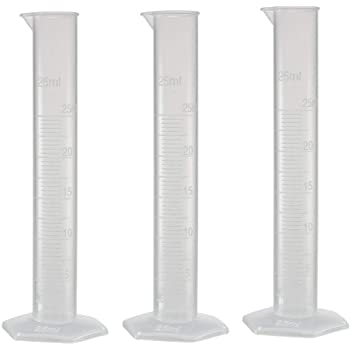
\includegraphics[width=5cm, height=5cm]{cylinders.jpg}
%%     \caption{Three graduated lab cylinders, corresponding to three
%%      eigenvectors. Prior precision eigenvalues not shown.}
%%     \label{fig:cylinder}
%% \end{figure}



\subsection{Answer to Question \ref{q:why}}\label{subsec:why}
Building on Theorem \ref{thm:char}, we can now give a compelling
explanation to the measurement clusterization we observed for the
inverse problem of the heat equation (Fig.~\ref{fig:eigenvectors}).

Consider $\fwd$ and $\prcov$ from \emph{the inverse problem of the
heat equation}. As before, we denote the eigenvalues of
$\fwd\prcov\fwd^*$ by $\lambda_j$. We input these eigenvalues into our
\emph{generic} model, and find a D-optimal design $\opt$ for our
generic model using Theorem \ref{thm:char}. In our generic model, the
measurements we take are best utilized in reducing uncertainty for the
first $k$ eigenvectors. So, a D-optimal design arising from our
\emph{generic model} completely avoids measuring eigenvectors $k+1$
and above.

Of course, in a real life problem --- such as the inverse problem of
the 1D heat equation --- it is likely impossible to find measurement
locations for which all eigenvectors $k+1$ and above are
zero. However, if the eigenvalues of $\fwd\prcov\fwd^*$ decay quickly
(recall the square-exponential decay for eigenvalues of the 1D heat
equation in eq.\eqref{eq:decay}), a D-optimal design will try to
balance measuring a small number (i.e.~$k$) of the leading
eigenvectors.

The abovementioned balance is explored in
Fig.~\ref{fig:eigenvectors}. We allow $m=4$ measurements in $\Omega =
[0,1]$ and observe that D-optimal measurement locations are clustered
at $x_1 = 0.31$ and $x_2 = 0.69$. Upon close inspection of the scaled
eigenvectors of $\fwd \prcov \fwd^*$, we first observe that
eigenvectors $3$ and above have negligible prior amplitude. Since we
only have $m=4$ measurements at our disposal, we interpret these
results, following Theorem \ref{thm:char}, as implying we should only
care about measuring the first and second eigenvectors. Then, we note
the D-optimal $x_1,x_2$ present a compromise between the amplitude of
the first and second eigenvectors. For example, a measurement at
$x=0.5$ would have ignored the second eigenvector altogether, since
the second eigenvector is zero at $x=0.5$.

Now we can understand measurement clusterization for the inverse
problem of the heat equation. A D-optimal design attempts to measure
the first $k$ eigenvectors of $\fwd \prcov \fwd^*$. But there may be
(spatial) limitations on where these $k$ eigenvectors have large
amplitude. For the inverse problem of the heat equation there are two
spatial locations that present a good compromise between the
amplitudes of the first and second eigenvectors, namely $x_1$ and
$x_2$ --- see Fig.~\ref{fig:eigenvectors}. We have $m=4$ measurements
at our disposal but only two spatial locations that are a good
compromise between the first and second scaled eigenvectors. Thus,
clusterization arises as a consequence of the pigeonhole principle.

\begin{figure}\label{fig:eigenvectors}
    \centering
    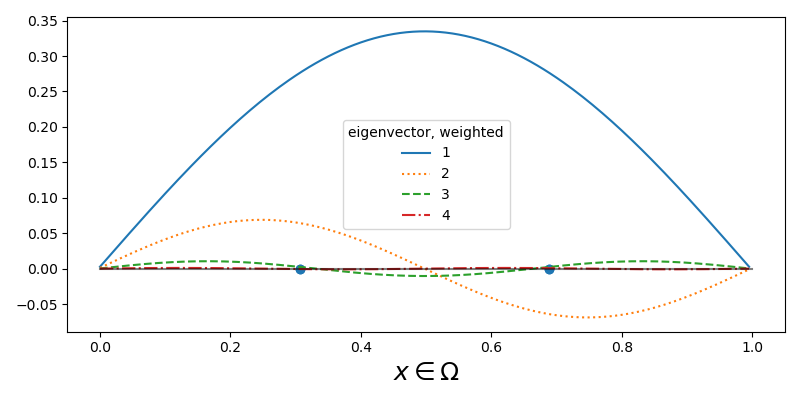
\includegraphics[width=\textwidth]{figs/eigenvectors_dst_scaled.png}
    \caption{D-optimal measurement locations ($m=4$ measurements) and
      weighted eigenvectors for finding the initial condition of the
      1D heat equation. Measurement locations and weighted
      eigenvectors are plotted over the computational domain $\Omega =
      [0, 1]$ (x-axis). Measurement clusterization occurs
      approximately at $0.31$ and $0.69$. These two locations are a
      compromise between the magnitudes of the first and second
      eigenvectors, which are the eigenvectors that a D-optimal design
      aims to measure. Allocating $m=4$ measurements into two
      locations results in clusterization, according to the pigeonhole
      principle.}
  \label{fig:why}
\end{figure}
